%! TEX root = **/000-main.tex
% vim: spell spelllang=en:

\section{NERC}%
\label{sec:nerc}

\subsection{Architecture}%
\label{sub:nerc-arch}

Our model layers have not deviated much from the original provided code.  show a visual representation of the model. We have several input layers, to which we apply embeddings. We then have a Dropout layer that helps avoid overfitting, and after that we just concatenate them.  The core of the computations is a bidirectional LSTM. Finally, a dense layer makes a prediction for each token in the sentence.


\subsection{Input information}%
\label{sub:nerc-input}

We decided to add several additional features as new inputs.  All of them were already used for the previous NERC assignment, so we will not go into detail explaining why they might be useful. 
\begin{itemize}
    \item \textbf{Words:} Basic token form.
    \item \textbf{Lowercased words:} Lowercased words. This was in part needed for the pretrained embeddings, as most of them store the token name lowercased.
    \item \textbf{Suffix:} Suffix of lengths 3 and 5
    \item \textbf{Lemma:} Lemma of words obtained by using a WordNetLemmatizer.
    \item \textbf{POS:} Part-of-speech of each word.
\end{itemize}

For each of them, we had to create indexes to encode them as numbers.

\subsection{Code}%
\label{sub:nerc-code}

\subsection{Experiments and results}%
Another important parameter we decided to experiment on is the number of epochs. The higher the number of epochs, the more the algorithm will pass through the entire training dataset, thus also increasing the computational time. Ideally, one should let the algorithm run for as long as there is no overfitting and the validation metrics keep improving.  

shows the evolution of accuracy and loss across several epochs. The training . This might suggest that we could stop training at around 3 epochs. Nevertheless, this could be a mistake as these plots can look quite different when changing some hyperparameter values, specially when modifying the learning rate, batch size or dropout rate. To better address this situation, we decided to use early stopping. More specifically, we will stop if the validation loss has not improved in 3 iterations.

\begin{figure}[H]
    \centering
    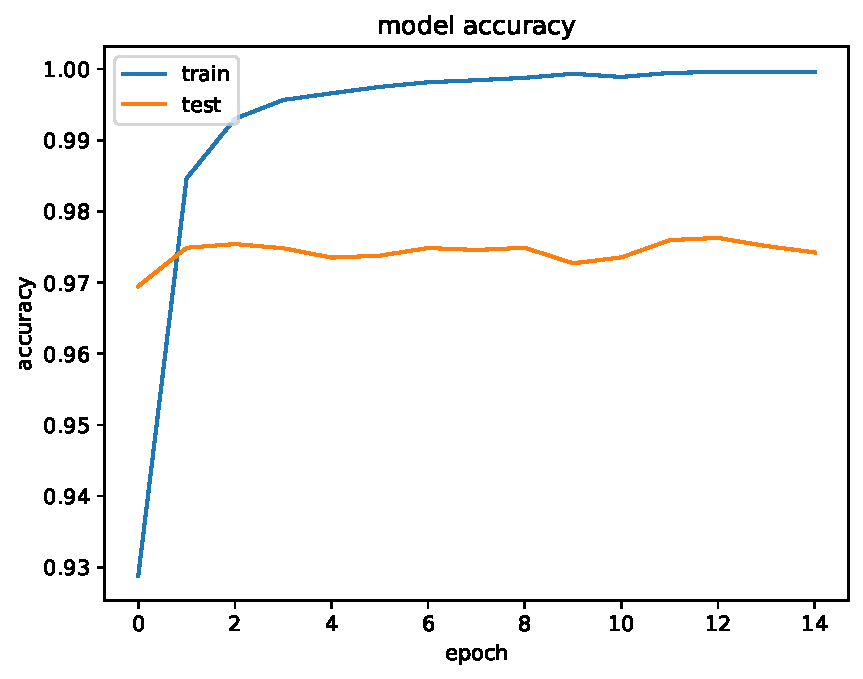
\includegraphics{figures/epoch-acc.pdf}
    \caption{Accuracy across epochs}
    \label{fig:epoch-acc}
\end{figure}

\begin{figure}[H]
    \centering
    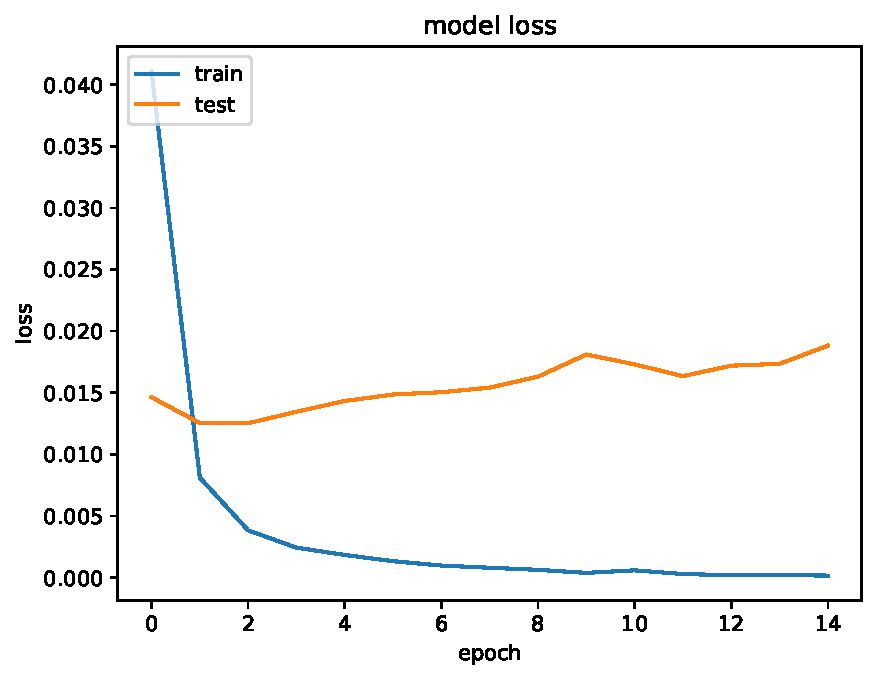
\includegraphics{figures/epoch-loss.pdf}
    \caption{Loss across epochs}
    \label{fig:epoch-loss}
\end{figure}


\subsubsection{Embeddings}
We also tried some pretrained embeddings like gloVe \cite{glove}, which is a model trained on the Wikipedia corpus that uses aggregated global word-word co-occurrence statistics to generate the embeddings. It provides embedding of 50d, 100d, 200d and 300d vector length. 

When using the Glove embeddings, we realized that there were many words in our training dataset that were not included. We attribute this to a not-perfect tokenization and to the fact that this model was trained using a general corpus and our data is subject specific.

To solve this issue, we also wanted to try to use a model that had been trained with a medical/pharmaceutical corpus. We found \href{https://github.com/ncbi-nlp/BioWordVec}{BioWordVec}, which is trained on the PubMed corpus and MeSH data and uses subword information to produce the embeddings. The resulting vectors are of dimension 200. As the file size is too large, it is impractical to read it each execution. To safe time, we just saved the train embedding matrix and loaded that instead.

As comparison, from our training data \textbf{TODO} were not found in gloVe, while only 2610 words were not present in BioWordVec. This could imply that the BioWordVec model might be a better fit for our data. Nevertheless, we tested this hypothesis by training different models using the different pretrained embeddings.



\label{sub:nerc-experiments}
